\section{Exploring the incidents' geographical distribution}
\label{sec:question1}

\subsection*{Question 1.1}
\textit{Are there high variations of incidents densities over Seattle? Which are the low-density zones? Which are the high density zones?}

The visualization uses a map of the city of Seattle (a scatter plot that uses the maps from OpenStreetMap for the background):
each point in the dataset is visualized as a circle on the map.
Columns and rows are used to encode respectively longitude and latitude.
The size of the circles is set to the minimum, the opacity to the value $8\%$.
Size and opacity do not encode any particular information.
However, the combination of small size, opacity and zoom level allows to visualize an approximation of the density of incidents.
The zoom level is small in order to get an overview of the entire city that fits the screen.
Size and opacity are adjusted accordingly.

\begin{figure}[h]
	\centering
	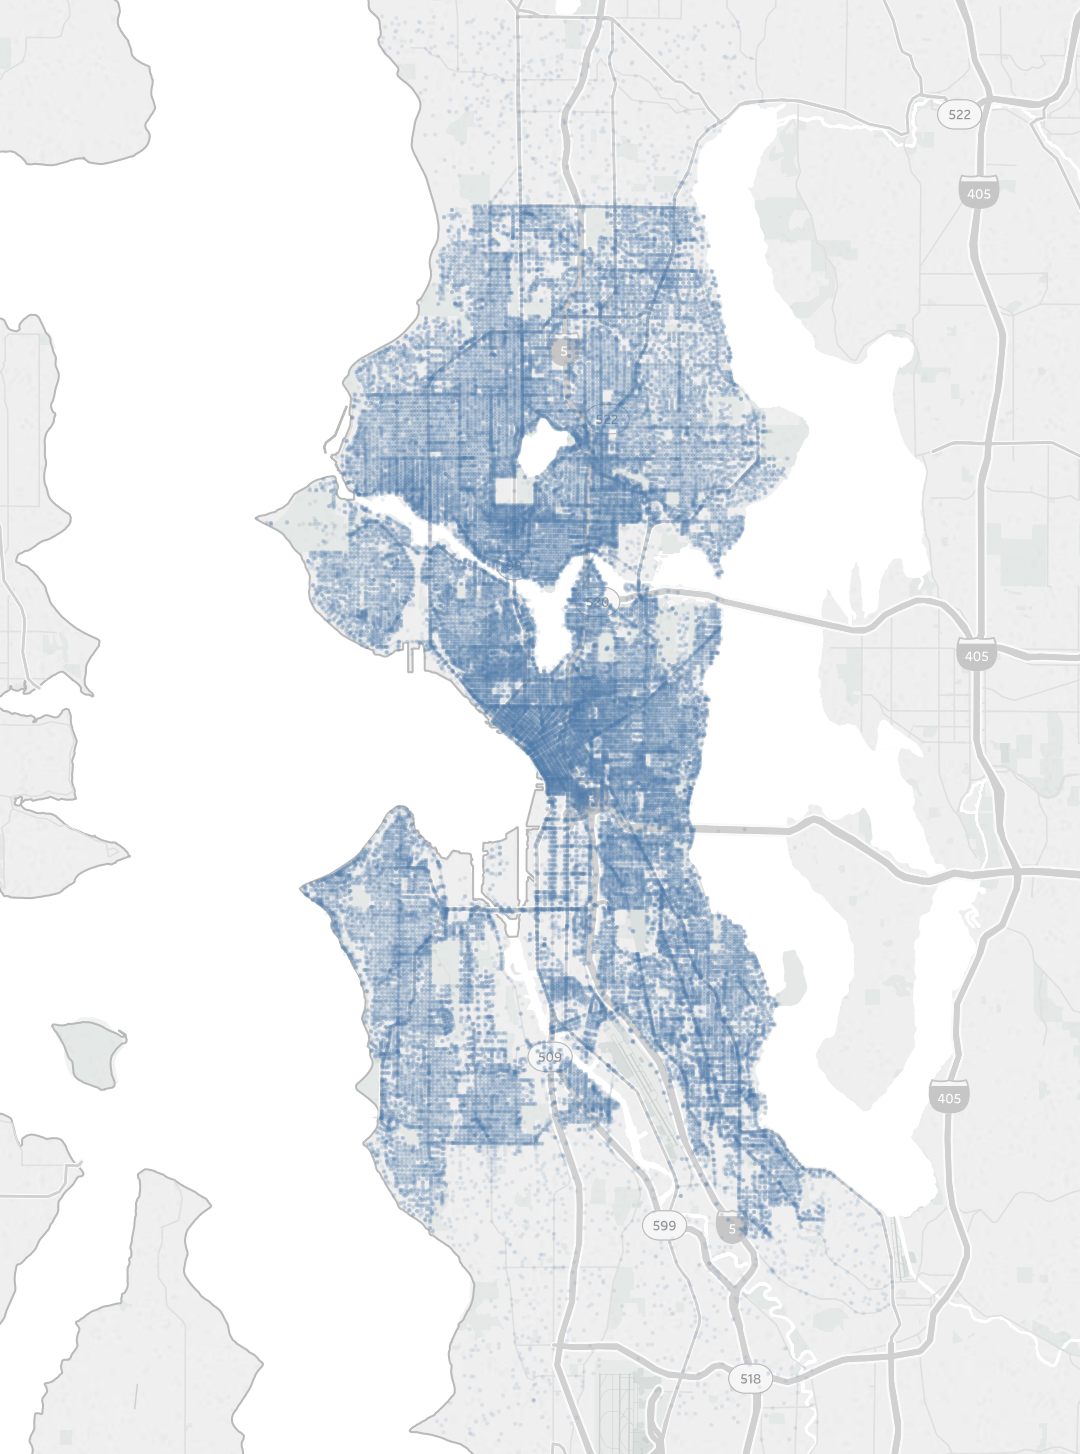
\includegraphics[width=.75\columnwidth]{figures/1_1_geographical_distribution_incidents}
	\caption{Geographical distribution of the incidents in Seattle. The screenshot is taken from the sheet called \textit{Geographical Distribution of Incidents in Seattle} in Tableau.}
	\label{fig:1_1_geographical_distribution_incidents}
\end{figure}

\cref{fig:1_1_geographical_distribution_incidents} shows that there are indeed variations in the density of incidents in Seattle:
\begin{itemize}
    \item The regions in the very north and south of the city have a very small number of incidents. These areas are already outside the borders of Seattle. We suspect they are not usually covered by the police of Seattle, so the dataset may not contain all the incidents that occurred in the those areas.
    \item Incidents seem to be more concentrated in the central area of the city, around the Elliott Bay, and immediately to its north.
    \item Outside the city center, the main roads have a higher number of incidents than the surrounding areas (in particular in the south part of the city).
    \item The density of incidents in the rest of the city is lower and seems to be approximately uniform.
\end{itemize}

The visualization answers the question, but it is not optimal.
A better solution would be to use a density plot which is able to visualize better the differences of incidents' densities in the city.
Unfortunately, Tableau does implement density plots: the proposed solution tries to approximate a density plot by finding the right level of opacity, size and zoom using Tableau.

\subsection*{Question 1.2}
\textit{Are there high variations of incidents densities over Seattle for specific types of incidents? Which are these types and which are the variations you found?}

\begin{figure}[h!] 
    \begin{subfigure}{0.5\textwidth}
        \centering
        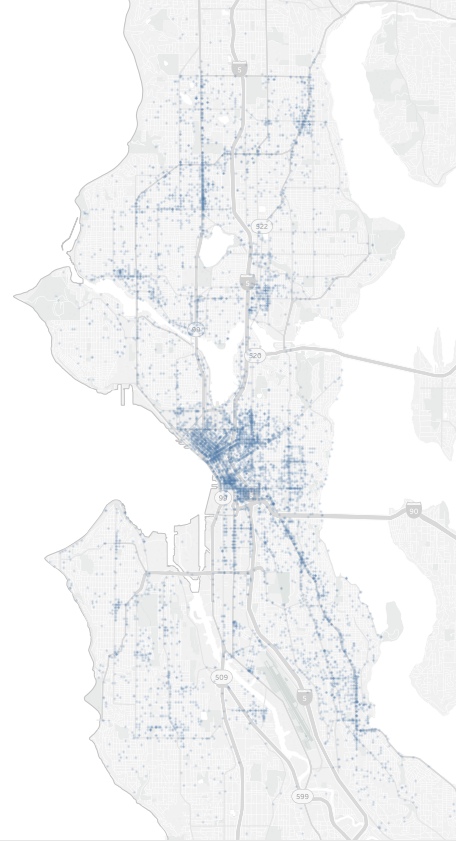
\includegraphics[width=0.8\linewidth]{figures/1_2_geographical_distribution_arrests} 
        \caption{Arrests}
        \label{fig:1_2_arrests}
    \end{subfigure}
    \begin{subfigure}{0.5\textwidth}
        \centering
        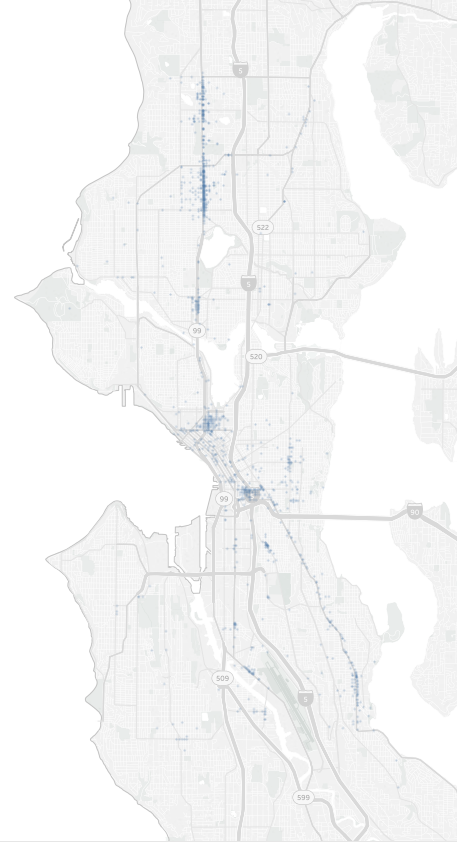
\includegraphics[width=0.8\linewidth]{figures/1_2_geographical_distribution_prostitution}
        \caption{Prostitution}
        \label{fig:1_2_prostitution}
    \end{subfigure}
    \caption{Geographical distribution of the incidents of type \textit{arrest} (on the left) and \textit{prostitution} (on the right) in Seattle. The screenshots are taken from the sheet called \textit{Sheet 22} in Tableau.}
    \label{fig:1_2_geographical_distribution_by_type}
\end{figure}

The visualization uses an approach similar to the previous section, but exploits pagination to display the different types of incidents individually.
This is done by using the ``Pages'' option in Tableau:
it is possible to interactively change the type visualized by using the dedicated menu.
The visualization uses a filter to exclude the observations without a type.
Since there are less observations in each page, the opacity value is set to a higher value ($30\%$).

\cref{fig:1_2_geographical_distribution_by_type} shows $2$ snapshots for the types \textit{arrest} and \textit{prostitution}.
From the figure it is already possible to notice that different types of incidents have different distributions in the city.
\cref{tab:distribution_by_type} contains the observations for every type of incident.

\renewcommand{\arraystretch}{1.5}
\begin{longtable}{ | >{\arraybackslash} m{5cm} | >{\arraybackslash} m{10cm} | }
    \hline
    \textbf{Incident Type} & \textbf{Description} \\
    \hline
    Accident Investigation  &   Higher concentration in the city center. Outside the city center, main roads have a higher concentration than the surrounding areas. \\
    \hline        
    Animal Complaints       &   Slightly higher concentration in the city center. \\
    \hline
    Arrest                  &   Higher concentration in the city center and along main roads in the north and south of the city. \\
    \hline
    Assaults                &   Like \textit{Arrest}. \\
    \hline
    Auto Thefts             &   No significant variations. \\
    \hline
    Behavioral Health       &   Higher concentration in the city center. \\
    \hline
    Bike                    &   Higher concentration in the city center. The north has a higher concentration thant the south. \\
    \hline
    Burglary                &   No significant variations. \\
    \hline
    Car Prowl               &   Slightly more concentrated in the city center. \\
    \hline
    Disturbances            &   Like \textit{Car Prowl}. \\
    \hline
    Drive By (No Injury)    &   Higher concentration in south east, almost absent in the other sectors. \\
    \hline
    Failure to Register (Sex Offender) &   Slightly more concentrated in the city center and south east. \\
    \hline
    False Alacad            &   No significant variations. \\
    \hline
    False Alarms            &   No significant variations. \\
    \hline
    Fraud Calls             &   Like \textit{Car Prowl}. \\
    \hline
    Harbor Calls            &   Concentrated along the coast. \\
    \hline
    Hazards                 &   Like \textit{Arrest}. \\
    \hline
    Homicide                &   Slightly more concentrated in the city center. \\
    \hline
    Lewd Conduct            &   Higher concentration in the city center. \\
    \hline
    Liquor Violations       &   Like \textit{Arrest}. \\
    \hline
    Miscellaneous Misdemeanors &   Like \textit{Arrest}. \\
    \hline
    Motor Vehicle Collision Investigation &   More concentrated in the center and along the streets. \\
    \hline
    Narcotics Complaints    &   Like \textit{Arrest}. \\
    \hline
    Nuisance, Mischief      &   Like \textit{Arrest}. \\
    \hline
    Other Property          &   Like \textit{Arrest}. \\
    \hline
    Person Down / Injury    &   Higher concentration in the city center. \\
    \hline
    Persons - Lost, Found, Missing &   Slightly more concentrated in the city center. \\
    \hline
    Property - Missing, Found    &   Slightly more concentrated in the city center. \\
    \hline
    Property Damage         &   Like \textit{Arrest}. \\
    \hline
    Prostitution            &   Concentrated along the main streets in the north and in the south. Present also in the city center. \\
    \hline
    Prowler                 &   No significant variations. \\
    \hline
    Public Gatherings       &   Higher concentration in the city center. \\
    \hline
    Reckless Burning        &   No significant variations. \\
    \hline
    Robbery                 &   Like \textit{Arrest}. \\
    \hline
    Shoplifting             &   Like \textit{Arrest}. \\
    \hline
    Suspicious Circumstances &   No significant variations. \\
    \hline
    Threats, Harassment     &   Like \textit{Arrest}. \\
    \hline
    Traffic Related Calls   &   No significant variations. \\
    \hline
    Trespass                &   Like \textit{Arrest}. \\
    \hline
    Vice Calls              &   No significant variations. \\
    \hline
    Weapon Calls            &   Like \textit{Arrest}. \\
    \hline

    \caption{Distribution of incidents in Seattle by type.}
    \label{tab:distribution_by_type}
\end{longtable}

The proposed visualization allows to analyze the distribution of incidents' types one by one.
However, it makes really difficult to compare different types, since the user needs to change page each time.

To overcome this limitation, we have to display different types together.
The first solution is to visualize all incidents together on the same map and use a categorical color map to distinguish them (see sheet \textit{Incidents Distribution (all types together)} in Tableau).
The user can interactively select subsets of types to display and filter out the others.
This solution presents $2$ main problems:
\begin{itemize}
    \item A categorical color map should use color which appear very different for each other to be useful, in the ideal case a set of color for which each pair has the same distance in RGB from each other. Unfortunately, it is impossible to find such a set for more than $4$ colors. We have about $40$ different types, so such an encoding is not effective.
    \item There are too many points, so even if we could find a good set of colors for the encoding, the point would overlap with each other. We can not use transparency to visualize also the underlying points since, since colors would mix together and create new ones.
\end{itemize}

One could use the following approaches to solve the problem:
\begin{itemize}
    \item Select a subset of types to show. Unfortunately, there is not an easy choice. Types with a higher number of incidents do not in general have an interesting distribution (i.e. their geographical distribution is similar to the one for all incidents). On the other hand, less frequent types have often a very interesting behaviour (see \textit{Prostitution}).
    \item Cluster similar types together. Unfortunately, it is not easy to build a types' hierarchy.
\end{itemize}

An alternative solution is to apply the small multiple design idea, i.e. create a visualization for a single type and replicate it multiple times.
This idea is implemented in sheet \textit{Incidents Distribution (small multiple design)} in Tableau:
each type is displayed on its own map, and maps for different types are shown in columns adjacent to each other (we use columns because the shape of the city on the chart is stretched out along the y-axis).
The type of incident in encoded both in space (different charts) and in color:
this overloading makes easier to distinguish different types.
Types are sorted in alphabetical order by default, but the user can interactively re-order them in order to compare $2$ or $3$ types at a time.
\cref{fig:1_2_geographical_distribution_comparison} shows an example of such a comparison:
types \textit{Prostitution}, \textit{Drive by} and \textit{Failure to register (self offender)} seem to be somehow correlated in the south-east part of the city but not in the north.
The size of each point is chosen to be small, but the opacity is set larger than for Question 1.1 since there are fewer point in each map.

\begin{figure}[h]
	\centering
	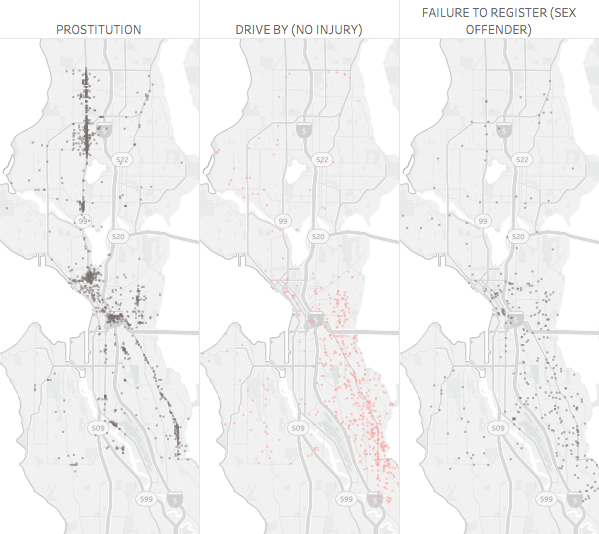
\includegraphics[width=.75\columnwidth]{figures/1_2_geographical_distribution_comparison}
	\caption{Geographical distribution of incidents of types \textit{Prostitution}, \textit{Drive by} and \textit{Failure to register (sex offender)} in Seattle. The screenshot is taken from sheet \textit{Incidents Distribution (small multiple design)} in Tableau.}
	\label{fig:1_2_geographical_distribution_comparison}
\end{figure}
